\documentclass{article}

\usepackage[left=2cm,right=2cm, top=2cm, bottom = 2cm]{geometry}
\usepackage{amsfonts}
%%%\usepackage{array}

\usepackage{tikz}

\pagestyle{empty}

\setlength{\tabcolsep}{15pt}
%%%\renewcommand{\arraystretch}{2.5}

%%%\makeatletter
%%%\newcommand{\thickhline}{%
%%%    \noalign {\ifnum 0=`}\fi \hrule height 2pt
%%%    \futurelet \reserved@a \@xhline
%%%}
%%%\newcolumntype{!}{@{\hskip\tabcolsep\vrule width 2pt\hskip\tabcolsep}}
%%%\makeatother

\begin{document}

\title{Location-Scale Transformations; Frequency, Amplitude, and Phase}
\date{}

\maketitle
\thispagestyle{empty}

\Large

{\bf \underline{Objective: To understand location-scale transformations of}}

\textbf{\underline{functions and their graphs, and the frequency, amplitude, and}}

\textbf{\underline{phase of a sinusoid.}}

\vspace{5mm}


{\bf Recap of previous material:}

\vspace{5mm}

Questions 1--6 are to be done without a calculator. Questions 7 and 8 may be left in exact form, or evaluated on a calculator for an approximate numerical answer.

\begin{enumerate}
\item What is $\sin(\sin^{-1}(0.1))$?
\item What is $\sin^{-1}\left(\sin\left(\frac{7\pi}{2}\right)\right)$?
\item What is $\cos(\cos^{-1}(-0.974))$?
\item What is $\cos^{-1}(\cos(-\pi))$?
\item What is $\tan(\tan^{-1}(-17))$?
\item What is $\tan^{-1}\left(\tan\left(\frac{3\pi}{4}\right)\right)$?
\item Convert the following points from cartesian to polar coordinates:
	\begin{enumerate}
	\item $(x,y)=(0,-3)$.
	\item $(x,y)=(-2,9)$.
	\item $(x,y)=(14,7)$.
	\end{enumerate}
\item Convert the following points from polar to cartesian coordinates:
	\begin{enumerate}
	\item $(r,\theta)=(0,2.017)$.
	\item $(r,\theta)=(3,\pi)$.
	\item $(r,\theta)=\left(7,\frac{7\pi}{4}\right)$.
	\end{enumerate}
\end{enumerate}


\clearpage

{\bf Warm-up:}

\vspace{5mm}

\begin{enumerate}
\item Let $f(x)=x^2+x$. Complete the following table:

\begin{tabular}{c|c|c|c|c|c|c|c}
$x$ & -3 & -2 & -1 & 0 & 1 & 2 & 3\\ \hline
$f(x)$ & & & & & & & \\ \hline
$f(x+1)$ & & & & & & & \\ \hline
$f(x-1)$ & & & & & & &
\end{tabular}


Hence identify which of the three curves below is $y=f(x)$, which is $y=f(x+1)$, and which is $y=f(x-1)$:

\begin{center}
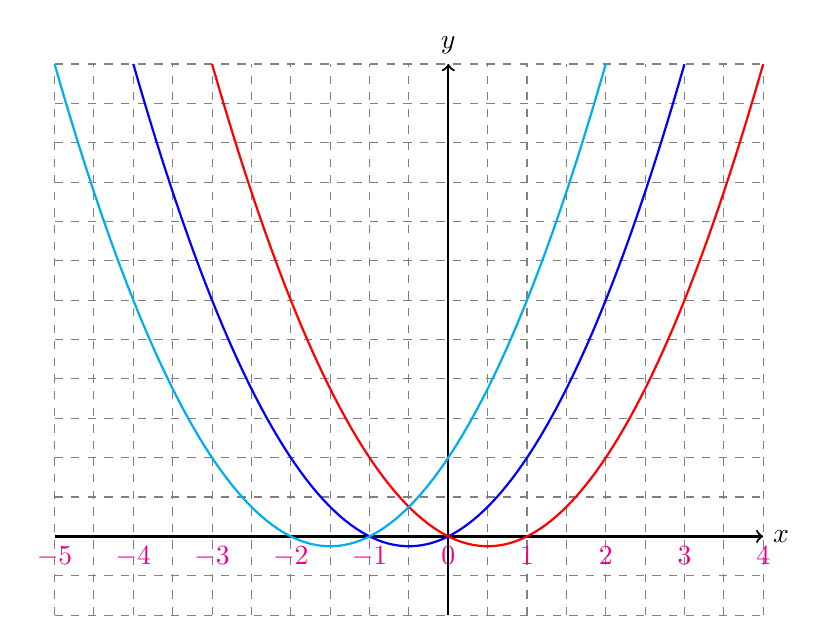
\begin{tikzpicture}
\draw[step=0.5,gray,thin,dashed] (-5,-1) grid (4,6);
\draw[thick, ->] (0,-1) -- (0,6);
\node[above] at (0,6) {$y$};
\draw[thick,->] (-5,0) -- (4,0);
\node[right] at (4,0) {$x$};

\draw[blue,thick, domain=-4:3, samples=100] plot (\x,{0.5*\x*(\x+1)});
\draw[red,thick, domain=-3:4, samples=100] plot (\x,{0.5*(\x-1)*(\x)});
\draw[cyan,thick, domain=-5:2, samples=100] plot (\x,{0.5*(\x+1)*(\x+2)});

\foreach \i in {-5, -4, -3, -2, -1, 0, 1, 2, 3, 4}{
	\node[below,magenta] at (\i,0) {$\i$};
	}
\end{tikzpicture}
\end{center}

\item Let $f(\theta)=\sin(\theta)$. Complete the following table:

\begin{tabular}{c|c|c|c|c|c|c|c|c|c}
$\theta$ & 0 & $\frac{\pi}{4}$ & $\frac{\pi}{2}$ & $\frac{3\pi}{4}$ & $\pi$ & $\frac{5\pi}{4}$ & $\frac{3\pi}{2}$ & $\frac{7\pi}{4}$ & $2\pi$\\ \hline
$f(\theta)$ & & & & & & & & &\\ \hline
$f(\theta)+1$ & & & & & & & & &\\ \hline
$f(\theta)-1$ & & & & & & & & &
\end{tabular}


Hence identify which of the three curves below is $y=f(\theta)$, which is $y=f(\theta)+1$, and which is $y=f(\theta)-1$:

\begin{center}
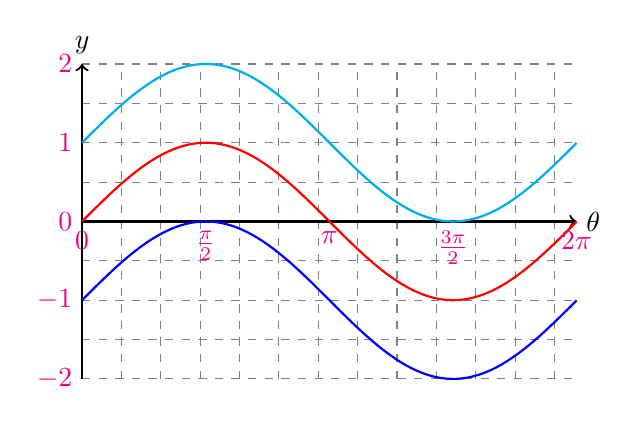
\begin{tikzpicture}
\draw[step=0.5,gray,thin,dashed] (0,-2) grid (6.28,2);
\draw[thick, ->] (0,-2) -- (0,2);
\node[above] at (0,2) {$y$};
\draw[thick,->] (0,0) -- (6.28,0);
\node[right] at (6.28,0) {$\theta$};

\draw[blue,thick, domain=0:6.28, samples=100] plot (\x,{sin(\x r)-1});
\draw[red,thick, domain=0:6.28, samples=100] plot (\x,{sin(\x r)});
\draw[cyan,thick, domain=0:6.28, samples=100] plot (\x,{sin(\x r)+1});

\node[magenta,below] at (0,0) {0};
\node[magenta,below] at (1.57,0) {$\frac{\pi}{2}$};
\node[magenta,below] at (3.14,0) {$\pi$};
\node[magenta,below] at (4.71,0) {$\frac{3\pi}{2}$};
\node[magenta,below] at (6.28,0) {$2\pi$};

\foreach \i in {-2,-1,0,1,2}{
	\node[left,magenta] at (0,\i) {$\i$};
	}
\end{tikzpicture}
\end{center}

\item Let $f(\theta)=\cos(\theta)$. Complete the following table:

\begin{tabular}{c|c|c|c|c|c|c|c|c|c}
$\theta$ & 0 & $\frac{\pi}{4}$ & $\frac{\pi}{2}$ & $\frac{3\pi}{4}$ & $\pi$ & $\frac{5\pi}{4}$ & $\frac{3\pi}{2}$ & $\frac{7\pi}{4}$ & $2\pi$\\ \hline
$f(\theta)$ & & & & & & & & &\\ \hline
$f(2\theta)$ & & & & & & & & &\\ \hline
$f\left(\frac{\theta}{2}\right)$ & & & & & & & & &
\end{tabular}

Hence identify which of the following curves is the graph of $y=f(\theta)$, which is $y=f(2\theta)$, and which is $y=f\left(\frac{\theta}{2}\right)$:

\begin{center}
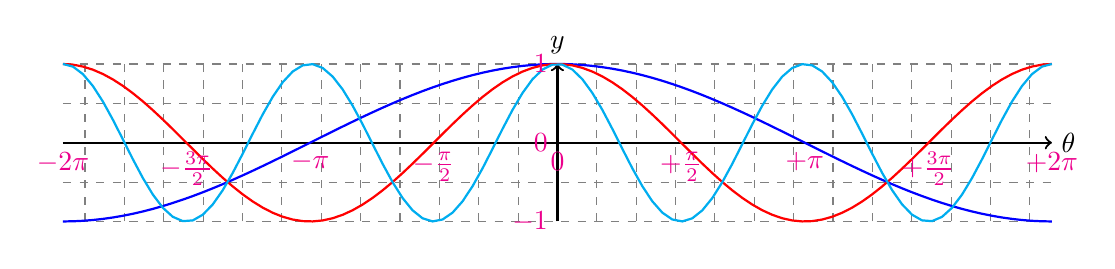
\begin{tikzpicture}
\draw[step=0.5,gray,thin,dashed] (-6.28,-1) grid (6.28,1);
\draw[thick, ->] (0,-1) -- (0,1);
\node[above] at (0,1) {$y$};
\draw[thick,->] (-6.28,0) -- (6.28,0);
\node[right] at (6.28,0) {$\theta$};

\draw[blue,thick, domain=-6.28:6.28, samples=100] plot (\x,{cos(\x/2 r)});
\draw[red,thick, domain=-6.28:6.28, samples=100] plot (\x,{cos(\x r)});
\draw[cyan,thick, domain=-6.28:6.28, samples=100] plot (\x,{cos(2*\x r)});


\node[magenta,below] at (0,0) {0};
\foreach \i in {+,-}{
	\node[magenta,below] at (\i1.57,0) {$\i\frac{\pi}{2}$};
	\node[magenta,below] at (\i3.14,0) {$\i\pi$};
	\node[magenta,below] at (\i4.71,0) {$\i\frac{3\pi}{2}$};
	\node[magenta,below] at (\i6.28,0) {$\i2\pi$};
	}
	
\foreach \i in {-1,0,1}{
	\node[left,magenta] at (0,\i) {$\i$};
	}
\end{tikzpicture}
\end{center}

\item Let $f(\theta)=\sin(\theta)$. Complete the following table:

\begin{tabular}{c|c|c|c|c|c|c|c|c|c}
$\theta$ & 0 & $\frac{\pi}{4}$ & $\frac{\pi}{2}$ & $\frac{3\pi}{4}$ & $\pi$ & $\frac{5\pi}{4}$ & $\frac{3\pi}{2}$ & $\frac{7\pi}{4}$ & $2\pi$\\ \hline
$f(\theta)$ & & & & & & & & &\\ \hline
$2f(\theta)$ & & & & & & & & &\\ \hline
$\frac{1}{2}f(\theta)$ & & & & & & & & &
\end{tabular}

Hence identify which of the following curves is the graph of $y=f(\theta)$, which is $y=2f(\theta)$, and which is $y=\frac{1}{2}f(\theta)$:

\begin{center}
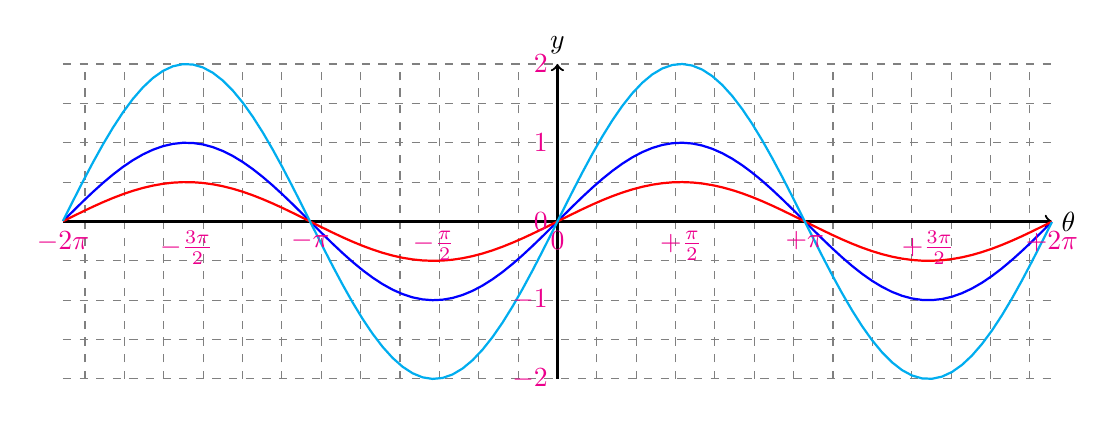
\begin{tikzpicture}
\draw[step=0.5,gray,thin,dashed] (-6.28,-2) grid (6.28,2);
\draw[thick, ->] (0,-2) -- (0,2);
\node[above] at (0,2) {$y$};
\draw[thick,->] (-6.28,0) -- (6.28,0);
\node[right] at (6.28,0) {$\theta$};

\draw[blue,thick, domain=-6.28:6.28, samples=100] plot (\x,{sin(\x r)});
\draw[red,thick, domain=-6.28:6.28, samples=100] plot (\x,{0.5*sin(\x r)});
\draw[cyan,thick, domain=-6.28:6.28, samples=100] plot (\x,{2*sin(\x r)});

\node[magenta,below] at (0,0) {0};
\foreach \i in {+,-}{
	\node[magenta,below] at (\i1.57,0) {$\i\frac{\pi}{2}$};
	\node[magenta,below] at (\i3.14,0) {$\i\pi$};
	\node[magenta,below] at (\i4.71,0) {$\i\frac{3\pi}{2}$};
	\node[magenta,below] at (\i6.28,0) {$\i2\pi$};
	}

\foreach \i in {-2,-1,0,1,2}{
	\node[left,magenta] at (0,\i) {$\i$};
	}
\end{tikzpicture}
\end{center}

\end{enumerate}




\clearpage


{\bf Theory --- Location Transformations:}

\vspace{5mm}

How are the graphs of the functions $y=f(x)$ and $y=f(x)+a$ related? How about $y=f(x)-a$?

\vfil

How are the graphs of the functions $y=f(x)$ and $y=f(x+a)$ related? How about $y=f(x-a)$?

\vfil


\clearpage

\textbf{Theory --- Scale Transformations:}

\vspace{5mm}

How are the graphs of the functions $y=f(x)$ and $y=af(x)$ related? How about $y=\frac{f(x)}{a}$?

\vfil

How are the graphs of the functions $y=f(x)$ and $y=f(ax)$ related? How about $y=f\left(\frac{x}{a}\right)$?


\clearpage


\textbf{Theory --- Amplitude, Frequency, and Phase:}

\begin{itemize}
\item A \textbf{sinusoid} is any curve obtained from the graph of $y=\sin(x)$ by a \textbf{location-scale transformation}.
\item The \textbf{amplitude} $A$ of a sinusoid is \textit{half} of the vertical distance between a maximum value (peak) and minimum value (trough):
	\begin{center}
	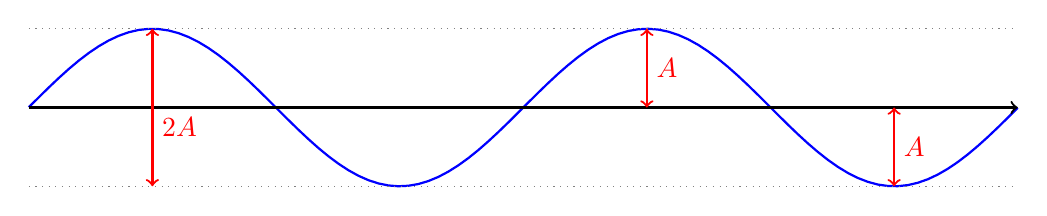
\begin{tikzpicture}
	\draw[blue,thick, domain=-6.28:6.28, samples=100] plot (\x,{sin(\x r)});
	\draw[thick,->] (-6.28,0) -- (6.28,0);
	\draw[dotted,gray] (-6.28,1) -- (6.28,1);
	\draw[dotted,gray] (-6.28,-1) -- (6.28,-1);
	
	\draw[red,thick,<->] (1.57,0) -- (1.57,1);
	\node[right,red] at (1.57,0.5) {$A$};
	\draw[red,thick,<->] (4.71,0) -- (4.71,-1);
	\node[right,red] at (4.71,-0.5) {$A$};
	\draw[red,thick,<->] (-4.71,1) -- (-4.71,-1);
	\node[below right,red] at (-4.71,0) {$2A$};
	\end{tikzpicture}
	\end{center}
\item The \textbf{period} $T$ (or \textbf{wavelength} $\lambda$) of a sinusoid is the horizontal distance between two adjacent peaks, or equivalently between two adjacent troughs. It is the distance after which the function repeats itself exactly:
	\begin{center}
	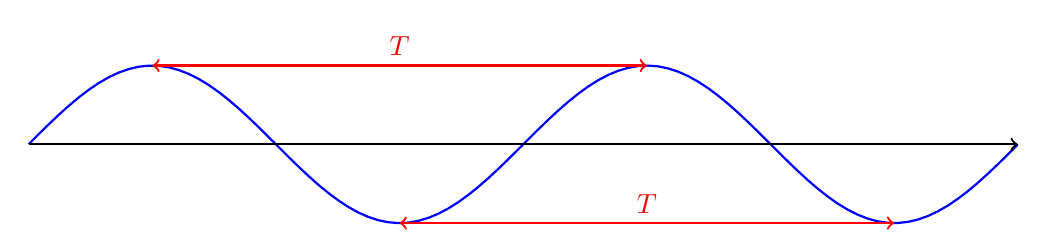
\begin{tikzpicture}
	\draw[blue,thick, domain=-6.28:6.28, samples=100] plot (\x,{sin(\x r)});
	\draw[thick,->] (-6.28,0) -- (6.28,0);
	
	\draw[red,thick,<->] (-4.71,1) -- (1.57,1);
	\node[red,above] at (-1.57,1) {$T$};
	\draw[red,thick,<->] (-1.57,-1) -- (4.71,-1);
	\node[red,above] at (1.57,-1) {$T$};
	\end{tikzpicture}
	\end{center}
	
	The distinction between wavelength and period isn't too important. Typically if the $x$-axis has units of distance, we say wavelength and denote it $\lambda$, whereas if it has units of time or angle, we say period and denote it $T$. For electronics purposes, the $x$-axis will typically be in units of time or angle. An example with units of distance would be sound waves, where the $x$-axis is position and the $y$-axis is pressure.
		
\item The \textbf{frequency} $f$ of a sinusoid is the reciprocal of the period:
	\[f=\frac{1}{T}.\]
	The frequency is the number of complete cycles the sinusoid goes through in one unit along the $x$-axis. Frequency is a natural measure when the $x$-axis has units of time; in this case, frequency has units of Hz ($\rm{s}^{-1}$). It is sometimes called \textbf{ordinary frequency} to distinguish it from:
	
\item The \textbf{angular frequency} $\omega$ of a sinusoid is the number of complete cycles the sinusoid goes through in $2\pi$ units along the $x$-axis. It is the natural measure when the $x$-axis is in radians. The relation between ordinary and angular frequency is given by
\[\omega=2\pi f.\]

An angular frequency in degrees would also be possible, and would be the number of complete cycles the sinusoid goes through in $360^\circ$; however, radians are essentially always used in technical applications.

\item The \textbf{phase} $\phi$ of a sinusoid is how far the sinusoid must be horizontally translated to line up with a normal sine wave, so that the sinusoid is increasing through the origin. The phase below is positive, as the sinusoid must be translated positively (to the right) to move the point at which it rises through the horizontal axis to the origin:
	\begin{center}
	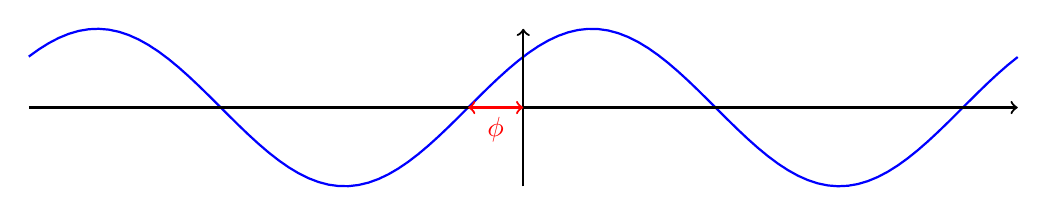
\begin{tikzpicture}
	\draw[blue,thick, domain=-6.28:6.28, samples=100] plot (\x,{sin((\x + 0.7) r)});
	\draw[thick,->] (-6.28,0) -- (6.28,0);
	\draw[thick,->] (0,-1) -- (0,1);
	
	\draw[red,thick,<->] (-0.7,0) -- (0,0);
	\node[red,below] at (-0.35,0) {$\phi$};
	\end{tikzpicture}
	\end{center}

The phase can actually be adjusted by adding any multiple of the period without changing the sinusoid. So the same sinusoid as above could be said to have the negative phase shown below:
	\begin{center}
	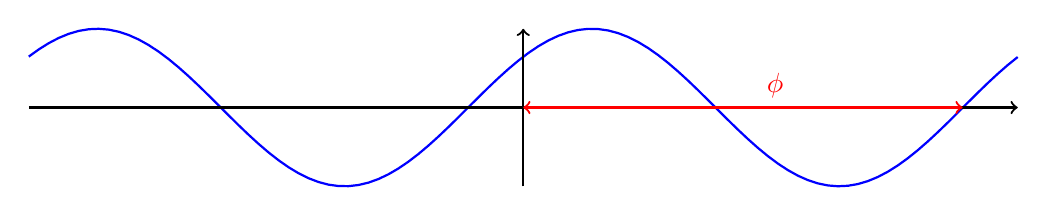
\begin{tikzpicture}
	\draw[blue,thick, domain=-6.28:6.28, samples=100] plot (\x,{sin((\x + 0.7) r)});
	\draw[thick,->] (-6.28,0) -- (6.28,0);
	\draw[thick,->] (0,-1) -- (0,1);
	
	\draw[red,thick,<->] (0,0) -- (5.58,0);
	\node[red,above] at (3.2,0) {$\phi$};
	\end{tikzpicture}
	\end{center}
	
	Typically we choose a range (either $0$--$2\pi$ or $-\pi$--$\pi$) and give the value of the phase in this range. However, in principle there are infinitely many different choices of phase that would give the same sinusoid, because $\phi+nT$ will do for any integer $n$.
\end{itemize}

Any sinusoid is a location-scale transformation of the standard sine wave, so has the form
\[y=A\sin(\omega t+\phi)+b\]
for some constants $A$, $b$, $\omega$, and $\phi$. Here $A$ is the \textbf{amplitude}, $\omega$ is the \textbf{angular frequency}, $\frac{\omega}{2\pi}$ is the \textbf{ordinary frequency}, and $\phi$ is the \textbf{phase}.

In many applications, $b$ can be taken to be 0---just set up your axes so that the midpoint of the oscillation is at $y=0$---but if we have non-zero $b$, we call it the \textbf{offset}. It is not generally very important, because of how easily it can be taken to be 0.



\clearpage

{\bf Practice:}

\vspace{5mm}

\begin{enumerate}
\item \begin{enumerate}
	\item Sketch the graph of $y=\cos(-\theta)$.
	\item Hence sketch the graph of $y=\cos\left(\frac{\pi}{2}-\theta\right)$.
	\item Give the amplitude and phase of this sinusoid.
	\item Compare this with the graph of $\sin(\theta)$. Explain this result using the definitions of sine and cosine.
	\end{enumerate}
\item \begin{enumerate}
	\item Sketch the graph of $y=x^2$.
	\item By completing the square, express $x^2-4x-12$ in the form $(x-a)^2+b$ for some constants $a$ and $b$.
	\item Hence sketch the graph of $y=x^2-4x-12$.
	\end{enumerate}
\item Sketch the graph of $y=\tan(x)$. Hence sketch the graph of $y=\tan\left(x+\frac{\pi}{4}\right)-1$.
\item Sketch the graph of $y=\cos(t)$. Hence sketch the graph of $y=2\cos(2t)$. Identify the amplitude, angular frequency, ordinary frequency, and phase of this sinusoid.
\item Sketch the graph of $z=\sin(t)$. Hence sketch the graph of $z=\frac{1}{2}\sin\left(2t-\frac{\pi}{4}\right)+1$. Identify the amplitude, frequency, angular frequency, phase, and offset of this sinusoid.
\item In the UK (and indeed the entire EU), mains electricity provides alternating current, such that the voltage $V$ delivered by a wall socket varies with time according to the equation
\[V=230\sqrt{2}\sin(100\pi t).\]
Identify the amplitude, frequency, and angular frequency of this sinusoid. Note: mains voltage is typically quoted as 230V; this is the ``root mean square'' value---a kind of average that's useful for power calculations, for instance. It's converting from this root mean square that causes the factor of $\sqrt{2}$ to appear in the above equation.

\end{enumerate}




\clearpage


{\bf Key Points to Remember:}

\vspace{5mm}

\begin{enumerate}
\item There are two \textbf{location transformations} we can apply to a graph $y=f(x)$:
	\begin{enumerate}
	\item The graph of $y=f(x+a)$ is obtained by shifting distance $a$ \textit{to the left}.
	\item The graph of $y=f(x)+a$ is obtained by shifting distance $a$ \textit{upwards}.
	\end{enumerate}
\item There are two \textbf{scale transformations} we can apply to the graph $y=f(x)$:
	\begin{enumerate}
	\item The graph of $y=af(x)$ is obtained by \textit{stretching vertically} by a factor of $a$.
	\item The graph of $y=f(ax)$ is obtained by \textit{squashing horizontally} by a factor of $a$ - equivalently, stretching by a factor of $\frac{1}{a}$.
	\end{enumerate}
\item A \textbf{sinusoid} is a sine wave after any location-scale transformation. It has equation
\[y=A\sin(\omega t+\phi)+b,\]
where $b$ is usually 0.
\item The \textbf{amplitude} $A$ is the vertical height the sinusoid reaches above (and below) the midpoint.
\item The \textbf{angular frequency} $\omega$ is the number of complete cycles the sinusoid makes every $2\pi$ units along the $t$-axis.
\item The \textbf{ordinary frequency} $f$ is $\frac{\omega}{2\pi}$.
\item The \textbf{phase} $\phi$ measures where in a cycle the sinusoid is at time 0; it is the amount the sinusoid must be horizontally translated by to pass through the origin while increasing (assuming no offset).
\end{enumerate}






\end{document}